\section{Introduction}

% Establish the teritory, the importance and reviewing previous work. how does this assignment relate to cyber-security

The life of a cyber-security professional can be a thankless task at times. Even with cyber-security spend increasing as a percentage of IT budgets \autocite{Hiscox:2022},
boards are reporting that they are not seeing eye-to-eye with their CISOs where \enquote{65\% of board members think their organization is at risk of a material
  cyberattack, only 48\% of CISOs share that view.} and that this \enquote{communication gap and board-CISO misalignment hinders progress in cybersecurity}
\autocite{Milica:2023}.

\begin{figure}[H] % Single column figure
  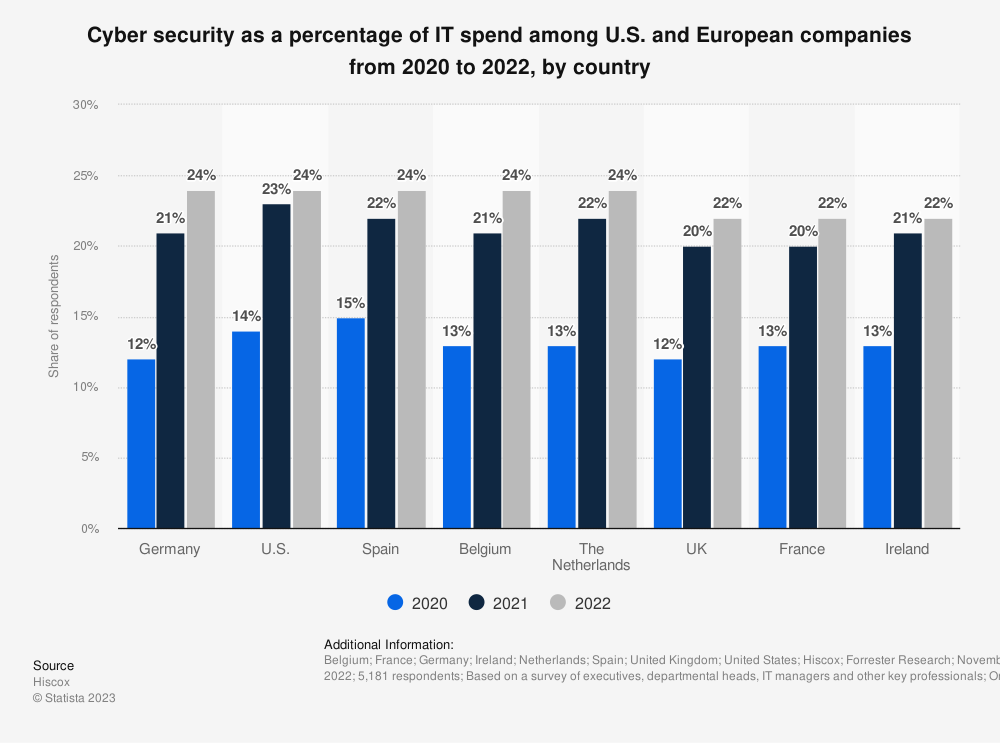
\includegraphics[width=0.5\textwidth]{statistic_id1245356_share-of-it-spend-on-cyber-security-in-the-us-and-europe-2020-2022-by-country.png}\hfill
  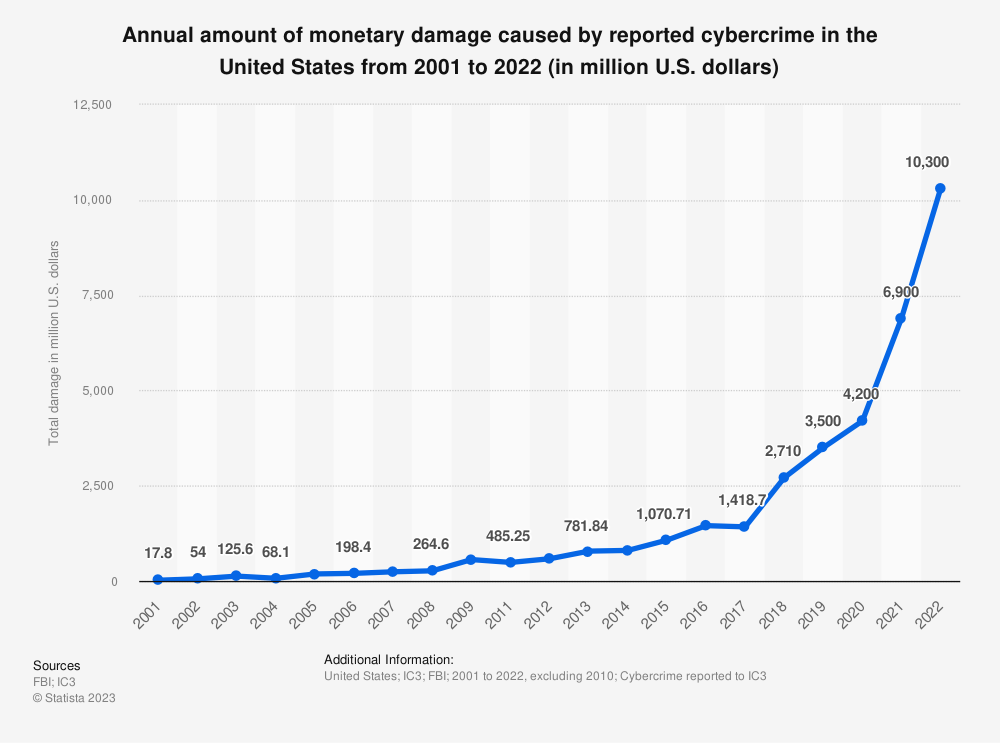
\includegraphics[width=0.5\textwidth]{statistic_id267132_annual-amount-of-financial-damage-caused-by-reported-cybercrime-in-us-2001-2022.png}\hfill

  \caption{Spending on Cyber Security  \autocite{Hiscox:2022} and Financial Damage caused by Cybercrime in the USA year-on-year \autocite{FBI:2023} Source: Statistica Inc.}
  \label{fig:cyber-spend-vs-cost}}
\end{figure}


It only takes a a few minutes for a new exploit to be found to get access to a companies computing assets.  Citrix recently reported a Netscaler Gateway code injection
vulnerability, \autocite{CVE-2023-3519}, as well as a privilege escalation attack \autocite{CVE-2023-3467}.  These are examples of novel attack vectors that  are
completely different to the normal social engineering attacks that corporate users are regularly trained to look for and avoid.  While protecing against a users of
email systems on clicking on a nefarious URL link, or opening a spreadsheet, there's rich buffet of choices, new and old, for an attacker to pick from when target
targeting a corporation's assets.

For organisations with assets that threat actors want to attack, it's necessary to at a minimum keep abreast of both reported Common Vulnerability and Exposures (CVE)
security flaws of their systems, published by NIST and MITRE, and reviewing advisories such as those issued by the Cybersecurity and Infrastructure Security Agency (CISA)
as ongoing cybersecurity education about groups such as ransomware gangs and their techniques \autocite{CISA:2023}.

% \href{https://www.cshub.com/attacks/articles/five-active-ransomware-gangs-and-their-tactics-part-one}{tactics} are a vital part of an organisation's cyber-security education and defence.

This cat-and-mouse game beween security groups on the one hand, and the evasion and increased sophistication and novelty on the part of malicious actors on the other \ldots
\textit{introduce EDR} \ldots
For vendors of EDR, MDR \& XDR solutions investigating existing and emerging threats is an on-going process \href{https://research.tue.nl/files/305661196/Olteanu_I.C..pdf}{evaluating the response effectiveness of their XDR technology}.

% Identify a niche, indicating a gap in in knowledge

Relying on EDR systems as a principle defence against a myriad of attacks alieviates many problems.  But it does not alievate the communication gap between company boards
and the cyber and information security professionals that protect their organisation.  CISOs need to understand the threat landscape, their mitigants to attacks, and
where failures in their own security systems may fail.  Having new internal analysis and being fully abreast of the threats, vulnerabilities and mitigants of their
systems will equip our CISO with the information they need to formulate and communicate a set of action/response readiness to the senior executives and board members. 

% Occupy the niche; purpose of new research, listing questions, the value of the work and the structure of the writing

This paper is a model for the types of analysis that a CISO should be requesting from their information security teams.  This paper reports on a new process injection technique \autocite{Peixoto:2023} in relation to the protections offered by EDR and XDR technologies, and specifically with behaviours that could be used to detect API attacks \autocite{Wang:2022}.

We will analyse the ``Mockingjay'' attack and identify the defences offered by modern XDR systems and ask if there's a credible chance of evading detection.  By looking at an implementation of the attack we will ask in what ways a threat detection system strengthen it's defences, and what artifacts could be automatically produced that could demonstrate any anomoly in a systems behaviour. 

Section 2 is a literature review of process injection attacks and endpoint security that is typically relied upon to prevent these types of attack.  We will then look at methods a identifying these attacks and look at the likelihood of Endpoint Security products of identifying the attack.

Section 3 an investigation into the Mockingjay attack and against a recently published paper ``Procguard'' \autocite{Wang:2022} and asks weather this attack method would lickly be caught.

% {jwang,mcj123,ZiangLi,2018302180148,iwangjye}@whu.edu.cn

Section 4 is an implementation of the attack and will look at manually identifying an infected process and generating artifacts that could be used in automating the process.

Section 5 is an evaluation section, reflecting on the project.

Section 6 is the conclusion and will suggest risks and mitigants for process injection attacks and further research that could be undertaken to use reinforcement to identify ``RWX'' code injections that should be part of a corporations EDR solution.

